\section{Introduction}
\label{sec:intro}
Two generators can have the same global variance while assigning very
different probabilities to parts of the image distribution. For a
few-step sampler, that difference determines what needs to change.
Changing the starting noise can recover image neighborhoods lost during
sampling. A digit that remains absent under several adequate samplers
calls for a test of the training distribution. The two cases require
different controls and different outcomes.

Existing occupancy tests can detect a change in a fixed region
\cite{richardson2018ndb}. To act on that change, we need to know how
large it is, what reference it is relative to, and whether an
intervention improves the target without violating fidelity criteria.
We fix the reference, regions, and effect sizes before evaluation.
A longer teacher sampler measures the change introduced by a faster
sampler. Observed data can reveal an imbalance shared by both.
Conditional spread then measures variation among samples in the same
region or under the same prompt.
\begin{figure}[t]
\centering
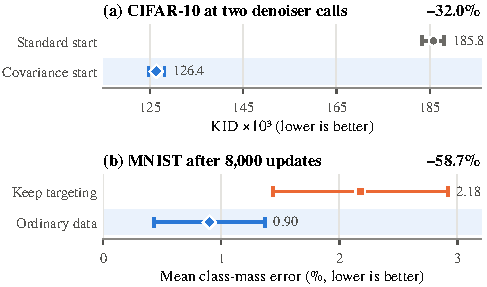
\includegraphics[width=\linewidth]{../figures/overview.pdf}
\caption{Reference-calibrated diagnosis enables independently verified repairs.
(a) Covariance initialization improves two-call CIFAR-10 Kernel Inception
Distance over five generated-sample panels from one checkpoint. (b) Ordinary
continuation reduces class-mass error in a separate equal-8,000-update
MNIST study across three training seeds. Whiskers show ordinary 95\%
Student-$t$ intervals.}
\label{fig:overview}
\end{figure}

Two confirmed repairs demonstrate this approach (Fig.~\ref{fig:overview}).
On CIFAR-10, covariance initialization reduces two-call Kernel Inception
Distance (KID) by 32.0\% and increases real-data DINO coverage from 0.206
to 0.288. Evaluating the same outputs against a separate CIFAR-10.1 reference
gives 32.7\% lower KID. On MNIST, signed regional measurements identify
overcorrection after targeted restoration. A separate equal-update
ordinary-data continuation lowers class-mass error by 58.7\% within the
declared fidelity margins.

Consider a reference with probabilities $(1/4,1/2,1/4)$ at feature
values $(-2,0,2)$ and a candidate with equal mass at $-\sqrt{2}$ and
$\sqrt{2}$. Both have mean zero and variance two. The fixed region
$[-1/2,1/2]$ contains half the reference mass and zero candidate mass.
If 100 independent draws per distribution give 50 reference hits and zero
candidate hits, the one-region audit gives a 97.5\% simultaneous upper
bound of 0.133 on the mass ratio. This certifies depletion at the
declared threshold of 0.5 (Sec.~\ref{sec:method}).

We ask three questions. Which regions lose or gain probability relative to
a fixed reference? How does variation within a region or prompt change
when fidelity is measured separately? Which controlled interventions
repair the diagnosed deficit on independent samples?

We contribute a fixed-reference audit that distinguishes regional loss,
within-region contraction, and departures from reference support. Its
finite-sample bounds show how the resolution of a regional diagnosis
depends on the effect size, reference mass, and comparison family.
We demonstrate two matched-budget repairs and explain why pooled
spread, within-prompt spread, and comparisons to different teachers
can give different answers about the same generator.
